\documentclass{beamer}[10]
\usepackage{pgf}
\usepackage[english]{babel}
\usepackage[utf8]{inputenc}
%\usepackage{beamerthemesplit}
\usepackage{graphics,epsfig, subfigure}
\usepackage{url}
\usepackage{srcltx}
\usepackage{hyperref}
\usepackage{physics}
\newcommand{\be}{\begin{equation}}
	\newcommand{\ee}{\end{equation}}
\newcommand{\bea}{\begin{eqnarray}}
	\newcommand{\eea}{\end{eqnarray}}
\newcommand{\rs}{r_{h}}
\usepackage{mathrsfs}

\usepackage{amsfonts}

\usepackage{bbm}

\usepackage{amsmath}

\usepackage{amssymb}

\usepackage{amsthm}

\usepackage{blkarray}

\usepackage{dsfont}

\usepackage{enumerate}

\usepackage{graphicx}

\usepackage{centernot}

\usepackage{caption}

\usepackage{braket}

\usepackage{slashed}

\usepackage{pgfplots}

\usepackage{feynmp-auto}

\usepackage{lastpage}
\newcommand{\dsum}[2]{\sum_{\substack{#1\\#2}}}
\newcommand{\dprod}[2]{\prod_{\substack{#1\\#2}}}
\usepackage{fancyhdr}
\usepackage[square,sort,comma,numbers]{natbib}

\usetikzlibrary{shapes.misc}

\tikzset{cross/.style={cross out, draw=black, minimum size=2*(#1-\pgflinewidth), inner sep=0pt, outer sep=0pt},
	%default radius will be 1pt. 
	cross/.default={2pt}}

\newcommand{\euler}[1]{\text{e}^{#1}}


\newcommand{\Real}{\text{Re}}

%For linespacing=1
\newcommand{\bbra}[2]{\left\langle\begin{matrix}\vspace*{-0.1cm}
		#2\\\vspace*{0.05cm}#1
	\end{matrix}\right\rvert}

\newcommand{\bket}[2]{\left\lvert\begin{matrix}\vspace*{-0.1cm}
		#2\\\vspace*{0.05cm}#1
	\end{matrix}\right\rangle}
\newcommand{\bbraket}[4]{\left\langle\begin{matrix}\vspace*{-0.1cm}
		#2\\ \vspace*{0.05cm}#1
	\end{matrix}\right\vert\left.\begin{matrix}\vspace*{-0.1cm}
	#4\\\vspace*{0.05cm}#3
\end{matrix}\right\rangle}

%\usepackage[all]{xy}


%For linespacing=1.5
%\newcommand{\bbra}[2]{\Big\langle\begin{matrix}\vspace*{-0.35cm}
%		#2\\\vspace*{0.15cm}#1
%	\end{matrix}\Big\rvert}
%
%\newcommand{\bket}[2]{\Big\lvert\begin{matrix}\vspace*{-0.35cm}
%		#2\\\vspace*{0.15cm}#1
%	\end{matrix}\Big\rangle}
%\newcommand{\bbraket}[4]{\Big\langle\begin{matrix}\vspace*{-0.35cm}
%		#2\\ \vspace*{0.15cm}#1
%	\end{matrix}\Big\vert\begin{matrix}\vspace*{-0.35cm}
%	#4\\\vspace*{0.15cm}#3
%\end{matrix}\Big\rangle}

\newcommand\Tstrut{\rule{0pt}{2.6ex}}         % = `top' strut
\newcommand\Bstrut{\rule[-0.9ex]{0pt}{0pt}}   % = `bottom' strut

\renewcommand{\ket}[1]{\left\lvert#1\right\rangle}
\renewcommand{\bra}[1]{\left\langle#1\right\rvert}
\newcommand{\sket}[1]{\left|#1\right]}
\newcommand{\sbra}[1]{\left[#1\right|}
\newcommand{\sbraket}[1]{\left[#1\right]}
\newcommand{\Span}[1]{\text{span}\left(#1\right)}
\newcommand{\MHV}{\text{MHV}}
\newcommand{\PT}{\text{PT}}
\newcommand{\Pf}{\text{Pf}}
\newcommand{\AMHV}{\mathcal{A}^{\MHV}}
\newcommand{\TAMHV}{\tilde{\mathcal{A}}^{\MHV}}
\newcommand{\MMHV}{\mathcal{M}^{\MHV}}
\newcommand{\ANMHV}{\mathcal{A}^{\text{N}\MHV}}
\newcommand{\MNMHV}{\mathcal{M}^{\text{N}\MHV}}
\newcommand{\Pfaff}[1]{\text{Pf}\left(#1\right)}
\newcommand{\rPfaff}[1]{\text{Pf}\ '\left(#1\right)}
\newcommand{\chyline}[2]{\draw[line width=0.5mm] (#1) -- (#2)}
\newcommand{\chydashedline}[2]{\draw[line width=0.5mm, dashed] (#1) -- (#2)}
\newcommand{\chydottedline}[2]{\draw[line width=0.5mm, dotted] (#1) -- (#2)}
\newcommand{\chydoubleline}[2]{\draw [double distance=0.9mm, line width=0.5mm] (#1) -- (#2)}

\newcommand{\chydoubledashedline}[2]{\draw [double distance=0.9mm, line width=0.5mm,dashed] (#1) -- (#2)}

\newcommand{\chytripleline}[2]{\chydoubleline{#1}{#2};\chyline{#1}{#2}
}

\newcommand{\chyquadrupleline}[2]{\draw [double distance=1.6mm, line width=0.5mm] (#1) -- (#2);
	\draw [double distance=0.3mm, line width=0.4mm] (#1) -- (#2)}

\newcommand{\chytripledashedline}[2]{\chydoubledashedline{#1}{#2};\chydashedline{#1}{#2}
}	

\newcommand{\polygonn}[2][]{
	\pgfmathsetmacro{\angle}{360/#2}
	\pgfmathsetmacro{\startangle}{-90-\angle/2}
	\pgfmathsetmacro{\y}{cos(\angle/2)}
	\tikzstyle{vertex}=[circle,fill=black,minimum size=7pt,text width = 7pt,inner sep=0pt]
	\foreach \i in {1,2,...,#2} {
		\pgfmathsetmacro{\x}{\startangle - \angle*\i}
		\node[vertex] (p\i) at (\x+\angle:1cm) [label={[label distance= -0.1mm]\x+\angle:$ \i $}] {};
	}
	
	
}
\newcommand{\polygonnn}[2][]{
	\pgfmathsetmacro{\angle}{360/#2}
	\pgfmathsetmacro{\startangle}{-90-\angle/2}
	\pgfmathsetmacro{\y}{cos(\angle/2)}
	\tikzstyle{vertex}=[circle,fill=black,minimum size=7pt,text width = 7pt,inner sep=0pt]
	\foreach \i in {1,2,...,#2} {
		\pgfmathsetmacro{\x}{\startangle - \angle*\i}
		\node[vertex,scale=0.1] (\i) at (\x+\angle:1cm) {};
	}
}
\newenvironment{polygon}[1][]
{	\def\myenvargumentII{#1} 
	\polygonnn{#1}}
{\polygonn{\myenvargumentII}
}

\newenvironment{chy}[1][]
{
	\begin{gathered}
		\begin{tikzpicture}[scale=0.65]
			\begin{polygon}[#1]
			}
			{
			\end{polygon}
		\end{tikzpicture}
	\end{gathered}
}



% TikZ til at lave figurer - for de avancerede
\usepackage{tikz}
% Div. pakker (muligt at ikke alle er i brug)
\usetikzlibrary{decorations.pathmorphing}
\usetikzlibrary{arrows.meta}
\usetikzlibrary{arrows}
\usetikzlibrary{decorations.pathreplacing,decorations.markings}
\usetikzlibrary{patterns}
\usetikzlibrary{fadings}
\usetikzlibrary{calc}
\usetikzlibrary{tikzmark,fit,shapes.geometric}

\definecolor{kugreen}{RGB}{79,112,148}
\definecolor{kugreenlys}{RGB}{255,242,204}
\definecolor{kugreenlyslys}{RGB}{173,190,177}
\definecolor{kugreenlyslyslys}{RGB}{214,223,216}
\setbeamercovered{transparent}
\mode<presentation>
%\usetheme[numbers,totalnumber,compress,sidebarshades]{PaloAlto}
\setbeamertemplate{footline}[frame number]
  \usecolortheme[named=kugreen]{structure}
  \useinnertheme{circles}
  \usefonttheme[onlymath]{serif}
  \setbeamercovered{transparent}
  \setbeamertemplate{blocks}[rounded][shadow=false]
  \setbeamercolor{block title}{bg=kugreen,fg=black}
	\setbeamercolor{block body}{bg=kugreenlys,fg=black}
\logo{
\includegraphics[width=1.4cm]{kuscience-logo}}
%\useoutertheme{infolines} 
\title{Black Hole Information Paradox}
\subtitle{An introduction}
\author{Taro Valentin Brown}
\institute{University of California, Davis}
\date{May 26, 2021.}
\setbeamercovered{invisible}

\begin{document}
\frame{\titlepage \vspace{-0.5cm}
}

\begin{frame}{Outline}{}
	\begin{itemize}
		\item Hawking's three points
		\item Hawking radiation
		\item Page Curve
		\item Suggested resolutions
	\end{itemize}
\vspace*{0.5cm}
References include
	\begin{itemize}
	\item Hawking's original paper [Phys. Rev. D 14, 2460]
	\item Reviews by 
	\begin{itemize}
		\item Polchinski [1609.04036]
		\item Raju [2012.05770]
		\item Hartman [\url{hartmanhep.net/topics2015/gravity-lectures.pdf}]
	\end{itemize}
\end{itemize}
\end{frame}
\section{Hawking's Paradox}
\begin{frame}{Hawking's Paradox}{Introduction}
	\begin{itemize}
		\item Hawking's paradox: 
		\\
		Evolving an initial state to a final state in a BH background turns a pure state into a mixed state. 
		\\
		From unitarity of quantum mechanics this is not allowed and points to information being lost. 
		\item We will look at Hawking's arguments and then see other versions of the paradox, e.g. Page curve.
	\end{itemize}
\end{frame}

\begin{frame}{Hawking's Paradox}{Intuition}
	\begin{itemize}
		\item First point:\\
		 Black holes are thermodynamic systems, with temperature, entropy etc. 
	\end{itemize}
"...black holes create and emit particles at a steady rate with a thermal spectrum. Because this radiation carries away energy, the black holes must presumably lose mass and eventually disappear."
\end{frame}

\begin{frame}{Hawking's Paradox}{Intuition}
	\begin{itemize}
		\item Can be seen even classically. Take Schwartzhild black hole
		\begin{equation}
			\begin{aligned}
				\dv{M_{BH}}{t}\propto -A T^{d+1}
			\end{aligned}
		\end{equation}
	Using dimensional analysis $m\propto r_h^{d-2}$, $T\propto r_h^{-1}$, and $A\propto r_h^{d-1}$:
		\begin{equation}
		\begin{aligned}
			\dv{r_{h}}{t}\propto -r_h^{-d+1}
		\end{aligned}
	\end{equation}
\item i.e. BH evaporates in time $t\propto r^{d}_h\propto \frac{A}{T}$
	\end{itemize}
\end{frame}

\begin{frame}{Hawking's Paradox}{Intuition}
	\begin{itemize}
		\item Second point:\\
 We need date from both $H$ and $\mathscr{I}^+$ to determine state initial on $\mathscr{I}^-$
	\end{itemize}
\end{frame}

\begin{frame}{Hawking's Paradox}{Intuition}
	\begin{itemize}
		\item Third point:\\
		This is also true quantum mechanically through hawking radiation.
		\item For simplicity, take Scwhartzhild metric in 1+1 dimensions (i.e. suppressing angular directions), a long time after the BH was formed, so no transient effects:
		\begin{equation}
			\begin{aligned}
				ds^2=-f(r)dt^2+\frac{dr^2}{f(r)},\;\;\;\;\;\;\; f(r)\equiv 1-\frac{r_h}{r}
			\end{aligned}
		\end{equation}
	\end{itemize}
\end{frame}

\begin{frame}{Hawking's Paradox}{Radiation}
	\begin{itemize}
		\item Transform coordinates to
		\begin{equation}
			\begin{aligned}
				\dd s^2=-f(r)\dd u \dd v=-\frac{4 r_h^2}{r}e^{-r/r_h}\dd U \dd V
			\end{aligned}
		\end{equation}
	with 
	\begin{equation}
		\begin{aligned}
		&r_*=r+r_h\log(r-r_h),\\ u=t-r^*=-2r_h&\log(-U/r_h),\;\;\; v=t+r^*=2r_h\log(V/r_h).
		\end{aligned}
	\end{equation}
\item $U,V$ are global coordinates. Smooth across horizon, so natural for an in-falling observer. 
\item $u,v$ are conformally related to $U,V$ and are only defined outside horizon.
	\end{itemize}
\end{frame}

\begin{frame}{Hawking's Paradox}{Radiation}
	\begin{itemize}
		\item Then consider a massless scalar field $\phi$, satisfying KG equation
		\begin{equation}
			\begin{aligned}
				\Box \phi =0
			\end{aligned}
		\end{equation}
	Will focus on the outgoing modes
	\bea
	\phi_{out} &=& \int_{0}^\infty \frac{d\nu}{2\pi(2\nu)^{1/2}}\, \left( a_\nu e^{-i\nu U} +a_\nu^\dagger e^{i\nu U} \right) \nonumber\\
	&=& \int_{0}^\infty \frac{d\omega}{2\pi(2\omega)^{1/2}}\, \left( b_\omega e^{-i\omega u} +b_\omega^\dagger e^{i\omega u} \right)   \,.
	\eea
	The nonzero canonical commutators are
	\be
	[ a_\nu, a_{\nu'} ] = 2\pi \delta(\nu-\nu')\,,\quad [ b_\omega, b_{\omega'} ] = 2\pi \delta(\omega-\omega') \,.
	\ee
	\end{itemize}
\end{frame}

\begin{frame}{Hawking's Paradox}{Radiation}
	\begin{itemize}
		\item From the mode expansion
		\be
		b_\omega = \int_{0}^\infty \frac{d\nu}{2\pi}\left( \alpha_{\omega\nu} a_\nu +  \beta_{\omega\nu} a_\nu^\dagger \right)\,, \label{atob}
		\ee
		where
		\bea
		\alpha_{\omega\nu} &=& 2\rs (\omega/\nu)^{1/2} (2 \rs\nu)^{2i  \rs \omega} e^{\pi  \rs \omega} \Gamma(- 2i  \rs \omega) \,, \nonumber\\
		\beta_{\omega\nu} &=& 2\rs (\omega/\nu)^{1/2}  (2 \rs\nu)^{2i  \rs \omega} e^{-\pi  \rs \omega} \Gamma(- 2i  \rs \omega) \,.
		\eea
	\end{itemize}
\end{frame}

\begin{frame}{Hawking's Paradox}{Radiation}
	\begin{itemize}
	\item \textbf{Reminder:} Adiabatic Principle. An in-falling observer sees the bh modes as empty, i.e.
	\begin{equation}
		\begin{aligned}
			a_\nu \ket{\psi}=0
		\end{aligned}
	\end{equation}
\item It follow from this that the occupation number for the $b_\nu$ modes is given by
\begin{equation}
	\begin{aligned}
		\langle \psi | b_\omega^\dagger b_{\omega'} | \psi \rangle= \frac{2\pi \delta(\omega-\omega')}{e^{\omega/T_{H}} - 1} 
	\end{aligned}
\end{equation}
\item I.e. we have a blackbody spectrum.
	\end{itemize}
\end{frame}

\begin{frame}{Hawking's Paradox}{Radiation}
	\begin{itemize}
		\item If one accounts for the modes incoming modes as well (labeled by $\tilde  b,\tilde b^\dagger$) one finds the final ground state
		\be
		\ket{\psi} = {\cal N} \exp \left( \int _0^\infty  \frac{d\omega}{2\pi} \, e^{- \omega/2T_{ H}}  b_\omega^\dagger \tilde b_\omega^\dagger \right)|0\rangle_{b,\tilde b},
		\label{bogo}
		\ee
	\end{itemize}
This is not a pure state!
\end{frame}

\begin{frame}{Hawking's Paradox}{Qbits}
	Thought experiment.
	\begin{itemize}
		\item Start with a pure state outside the BH consisting of $n$ entangled qubit pairs (EPR pairs).
		\item One part of the state goes into the BH and the other state reaching future null infinity.
		\item $\rho_{out}$ is mixed and so the entropy $S_{out} \sim n\log(2)$.
		\item After BH is completely evaporated, the entanglement doesn't decrease because of causality and so we are left with
		\begin{equation}
			\begin{aligned}
				S_{E} \sim n\log(2)
			\end{aligned}
		\end{equation}
	\end{itemize}
\end{frame}

\begin{frame}{Hawking's Paradox}{Unitarity}
	\begin{itemize}
		\item We went from a pure state to a mixed state under time evolution. Not coherent with quantum mechanics.
		\begin{equation}
			\begin{aligned}
				\rho^{ final}_{mm'} = S \hspace{-7pt} /_{mm',nn'}\rho^{initial}_{nn'} \,,
			\end{aligned}
		\end{equation}
		\item Hawking argued that since “information ... requires energy”, all the information about
		the initial state cannot emerge in the final stages of black hole evaporation. 
	\end{itemize}
\end{frame}

\begin{frame}{Page curve}{}
	\begin{itemize}
		\item Another way to view the paradox, using the Page curve.
	\end{itemize}
\end{frame}

\begin{frame}{Page curve}{Second law of thermodynamics}
	\begin{itemize}
		\item Beckenstein-Hawking entropy
		\begin{equation}
			\begin{aligned}
				S_{BH}=\frac{A_h}{4}
			\end{aligned}
		\end{equation}
		\item Generalized (coarse-grained) entropy
		\begin{equation}
			\begin{aligned}
				S_{gen}=S_{BH}+S_{outside}
			\end{aligned}
		\end{equation}
	\item Fine-grained entropy
	\begin{equation}
		\begin{aligned}
			S_{fine} = -\Tr[\rho \log \rho]
		\end{aligned}
	\end{equation}
		\item Further
		\begin{equation}
			\begin{aligned}
				S_{coarse}\geq S_{fine}
			\end{aligned}
		\end{equation}
	\end{itemize}
\end{frame}

\begin{frame}{Page curve}{}
		\centering 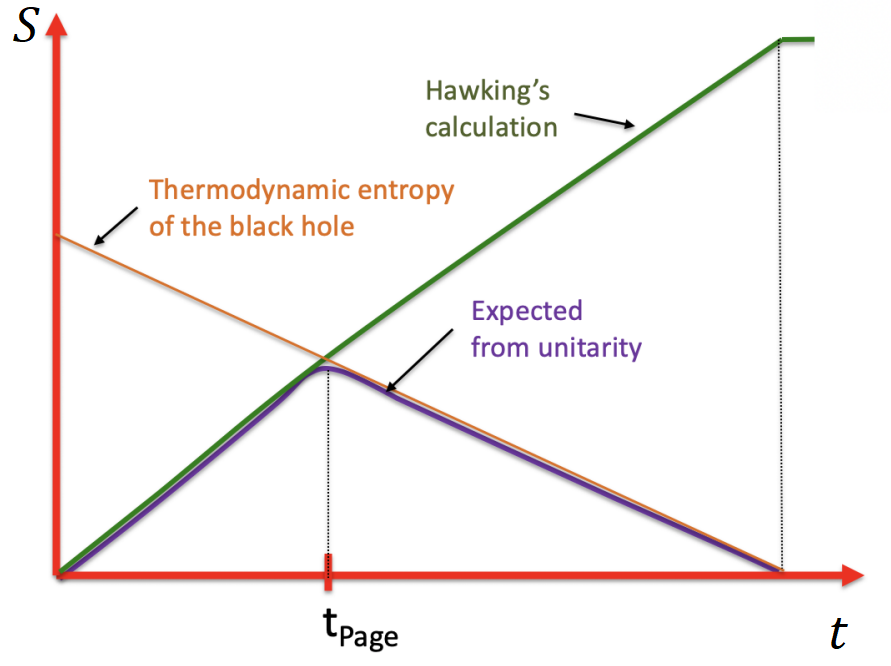
\includegraphics[width=7cm]{Page.png}		\vspace*{1cm}\newline
\end{frame}

\begin{frame}{Resolutions}{}
Three broad possibilities
\begin{itemize}
\item Calculation is correct and information is lost. \\
This breaks quantum mechanics/unitarity.
\item Hawking radiation contains all the information. \\ It seems to point at our EFT breaking down.
\item Remnants, i.e. BH doesn't shrink all the way, containing information that is still entangled. \\ 
We could have started with an arbitrarily large black hole, so
the number of states that must be available to this Planck-sized remnant is unbounded above
\end{itemize}
\end{frame}

\begin{frame}{Problems}{}
Some problems
	\begin{itemize}
		\item Calculation of $\rho$  is not exact
		\begin{equation}
			\begin{aligned}
				\rho=\rho^{thermal}+\text{ loops }+\mathcal{O}\left(e^{-S}\right)
			\end{aligned}
		\end{equation}
	\item If the number of terms in entropy is of size $e^{S}$, then these corrections could correct this and make the final state pure.
	\item Probably can not answer this in low energy EFT, so we need some UV theory.
	\item Hartman and collaborators argue that one can get a unitary entropy curve using low energy EFT. 
	\end{itemize}
\end{frame}

\begin{frame}
	\centering
	\Large Thank you for your attention.\\
\end{frame}		
\begin{frame}{Bonus slides}{Back reaction}
\be
b_\omega = R_\omega c_\omega + T_\omega \int_{0}^\infty \frac{d\nu}{2\pi}\left( \alpha_{\omega\nu} a_\nu +  \beta_{\omega\nu} a_\nu^\dagger \right)\,. \label{bca}
\ee
$c_\omega$ are left-moving modes, coming in from spatial infinity ${\mathscr I}^-$. \\
 $R_\omega$ is the amplitude for them to reflect before reaching the horizon and $T_\omega$ is the transmission amplitude, with $|R_\omega|^2 + |T_\omega|^2 = 1$. 
\be
\langle \psi | b_\omega^\dagger b_{\omega'} | \psi \rangle = |T_\omega|^2 \frac{2\pi \delta(\omega-\omega')}{e^{\omega/T_{ H}} - 1} \,. \label{grey}
\ee
\end{frame}		

\begin{frame}{Bonus slides}{Entropy}
	Types of entropy
	\begin{itemize}
		\item Von Neumann/fine-grained entropy
		\begin{equation}
			\begin{aligned}
				S(\rho)=-\Tr(\rho\log \rho)
			\end{aligned}
		\end{equation}
		Vanishes in a pure state and constant under unitary evolution.
		\item Coarse-grained entropy. Measure a subset of observables. Consider all density matrices which gives the same result as $\rho$ for our observables, and then maximize over the entropy
		\begin{equation}
			\begin{aligned}
				S(\tilde \rho;E,\dots)=\max_{\tilde \rho;E,\dots=\rho}[S(\tilde\rho)]\geq S(\rho)
			\end{aligned}
		\end{equation}
	\end{itemize}
\end{frame}

\begin{frame}{Page curve}{Second law of thermodynamics}
	\begin{itemize}
		\item 	Captured in spirit by
		\begin{equation}
			\begin{aligned}
				S\sim \min[\frac{A_h}{4}+S_{outside}]
			\end{aligned}
		\end{equation}
		\item Rather, take a Cauchy spatial slice and find a minimal surface. Then take the maximum of all the slices found, if there are multiple. Then
				\begin{equation}
			\begin{aligned}
				S= \min_X[\text{ext}_X[\frac{A(X)}{4}+S_{semi-cl}(\Sigma_X)]]
			\end{aligned}
		\end{equation}
	\end{itemize}
\end{frame}

\begin{frame}{Page curve}{Second law of thermodynamics}
	\centering \includegraphics[width=6cm]{Island1.png}		\vspace*{1cm}\newline
\end{frame}
\begin{frame}{Page curve}{Second law of thermodynamics}
	\centering \includegraphics[width=6cm]{Island2.png}		\vspace*{1cm}\newline
\end{frame}
\begin{frame}{Page curve}{Second law of thermodynamics}
	\centering \includegraphics[width=11.5cm]{Island3.png}		\newline
	\begin{equation}
		\begin{aligned}
				S= \min_X[\text{ext}_X[\frac{A(X)}{4}+S_{semi-cl}(\Sigma_{Rad}\cup \Sigma_{Island})]]
		\end{aligned}
	\end{equation}
\end{frame}
\end{document}
